\newpage~\\
\section{Versionskontrolle: git und GitHub}

Was ist Versionskontrolle?
\begin{itemize}
	\item Ein System, das Änderungen an Dateien im Laufe der Zeit aufzeichnet, sodass bestimmte Versionen später wieder hergestellt werden können.
	\item Engl.: Version Control System (VCS)
\end{itemize}
%
~\\
Warum ist das für uns interessant?
\begin{itemize}
	\item Fehlersuche: Wir können jede vorgenommene Änderung im Zeitverlauf überprüfen und ggf. einen früheren (hoffentlich stabilen) Zustand (snapshot) wiederherstellen.
	\item Kollaboration: Wir können zusammen an einem Projekt arbeiten und unabhängige Beiträge zum Code verwalten.
\end{itemize}
~\\
Was ist git?
\begin{itemize}
	\item git ist ein VCS und der de facto Standard
	\item Ursprünglich entwickelt von Linus Torvalds im Jahr 2005 für die Entwicklung des Linux-Kernels:\\ \url{https://www.youtube.com/watch?v=o8NPllzkFhE?t=07m40s}
	\item git ist ein verteiltes Versionskontrollsystem: Jeder Benutzer klont eine Kopie des Projekts und hat den gesamten Verlauf auf seiner eigenen Maschine.
	\item Der Ruf von git:
	\begin{figure}[h!]
		\centering
		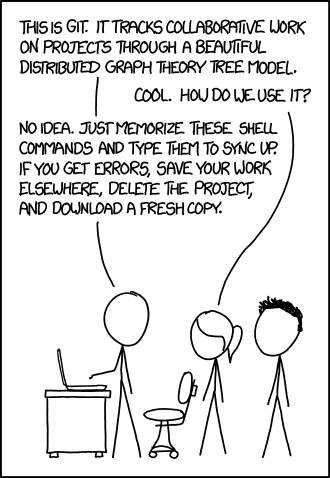
\includegraphics[width=0.3\linewidth]{media/git}
		\caption{\url{https://xkcd.com/1597/}}
		\label{fig:git}
	\end{figure}
\end{itemize}







\subsection{git}
[Tafel: DAG aufbauen]\\~\\
\textbf{Datenmodell}\\
\begin{itemize}
	\item \texttt{blob} : Datei
	\item \texttt{tree} : Verzeichnis
	\item \texttt{commit} : snapshot of top-level tree (immutable!)
	\begin{itemize}
		\item Date
		\item Author
		\item Message
		\item Parent
	\end{itemize}
	\item Historie wird gespeichert als gerichteter azyklischer Graph (\href{https://en.wikipedia.org/wiki/Directed_acyclic_graph}{directed acyclic graph (DAG)}): gerichteter Graph ohne gerichtete Zyklen (z.B. Stammbäume)
	\begin{itemize}
		\item Knoten = \texttt{commits}
		\item Kanten = Verwandtschaftsbeziehung (genauer: (x,y) := "commit y kommt vor \texttt{commit} x")
	\end{itemize}
	\item \texttt{object} : blob | tree | \texttt{commit}
	\begin{itemize}
		\item git speichert objects mithilfe ihrer SHA-1 Hashwerte (20 Bytes bzw. 40 Hexadezimalzahlen)
	\end{itemize}
	\item \texttt{references} = menschenlesbare Namen für Hashwerte von \texttt{commits} (also Zeiger auf Knoten im Graphen)
	\begin{itemize}
		\item Beispiele:
			\begin{itemize}
			\item  \texttt{master}/\texttt{main}: typischerweise letzter commit im Hauptzweig
			\item \texttt{HEAD}: commit der dem aktuellen lokalen Zustand entspricht\\
			$\rightarrow$ Wichtig, da neue commits den Graphen vom aktuellen commit als Startpunkt aus erweitern\\
			$\rightarrow$ Daher spricht man auch nicht von Benamung, sondern von Abzweigung/Verästelung (branching)
		\end{itemize}
		\item Drei Varianten von \texttt{references}:
		\begin{itemize}
			\item local \texttt{branch}
			\item remote \texttt{branch}
			\item \texttt{tag} = \texttt{reference}, die sich nicht bewegt (für Softwareversionen)
		\end{itemize}
	\end{itemize}
	\item \texttt{repository} : Vereinigung von allen \texttt{objects} und \texttt{references}
	\begin{itemize}
		\item Das ist im Wesentlichen alles was git auf der Festplatte speichert (in \texttt{.git})
	\end{itemize}
\end{itemize}
~\\
\textbf{Staging area:} Wie erstellen wir \texttt{commits}? 
\begin{itemize}
	\item Eine Möglichkeit: Snapshot (\texttt{commit}) auf der Grundlage des aktuellen Zustands des Projektverzeichnisses erstellen.
	\item Warum das zu grobkörnig ist:
	\begin{itemize}
		\item Beispiel 1: Angenommen wir haben zwei verschiedene Features implementiert und wollen dafür zwei \texttt{commits} erstellen, wobei der erste das erste Feature einführt und der nächste das zweite. 
		\item Beispiel 2: Angenommen wir haben print-Anweisungen zum Debuggen eingefügt, zusammen mit einer Fehlerbehebung. Wir möchten die Fehlerbehebung committen, während wir alle Druckanweisungen verwerfen.
	\end{itemize}
\item git erlaubt durch einen Mechanismus namens ``staging area'' festzulegen, welche Änderungen in den nächsten Snapshot (\texttt{commit}) aufgenommen werden sollen.
\end{itemize} 

~\\
\textbf{git verwenden: CLI}\\~
[Demo und Hands-On]\\
Alle Git-Befehle entsprechen letztlich einer Manipulation des \texttt{commit}--DAG durch Hinzufügen von Objekten und Hinzufügen/Aktualisieren von Referenzen.


\begin{itemize}
	\item \texttt{git init}: erstellt ein neues git repo, dessen Daten (\texttt{objects} und \texttt{references}) im Verzeichnis .git gespeichert werden
\item	\texttt{git status}: gibt Auskunft über den aktuellen Stand der Dinge
\item	\texttt{git add [FILENAME]}: fügt Dateien zur staging area hinzu
\item	\texttt{git commit -m <MESSAGE>}: erstellt neuen commit
\item \texttt{git log --oneline --abbrev-commit --all --graph --decorate --color}: Zeigt Veränderung (in Graphenansicht)
\item \texttt{branch} and \texttt{merge}: Erstellen von \texttt{references}
\begin{itemize}
	\item \texttt{git branch <branchname> [<start-point>]}\\
	-- \texttt{<branchname>} Name für den commit des aktuellen Zustandes oder für den commit \texttt{<start-point>}\\
	-- \texttt{<start-point>} ist optional (\texttt{branch}, \texttt{tag}, \texttt{hash\_value})
	\item Mal in \texttt{.git/refs/heads} schauen: wir schreiben lediglich eine Textdatei mit 40 Hex-Zahlen (das geht sehr schnell)
	\item Wir können Zweige zusammenbringen, in dem wir zwei \texttt{commits} verkleben\\
	\texttt{git merge}
\end{itemize}
\item \texttt{git checkout <commit>} : aktuelles Verzeichnis gemäß des commits \texttt{<commit>} herstellen, also Update von \texttt{HEAD}\\
-- \texttt{<commit>} ist optional (\texttt{branch}, \texttt{tag}, \texttt{hash\_value})
\end{itemize}








\subsection{GitHub}
\textbf{Situation}
\begin{itemize}
	\item Mehrere Entwickler arbeiten zusammen an einem Projekt.
	\item Das bedeutet: Es bestehen mehrere Klone des Projekts auf den lokalen Platten der Entwickler.
	\item Den Kunden möchte man allerdings nur einen Ort als Quelle angeben
	\item Dafür gibt es sogenannte \texttt{remote}--Repositories: Ein gemeinsames Repository, das alle Entwickler zum Austausch ihrer Änderungen verwenden (Pivot-Repo). 
	\item In den meisten Fällen wird ein solches Remote-Repository auf einem Code-Hosting-Dienst wie GitHub oder auf einem internen Server gespeichert.
\end{itemize}
%
\textbf{Remotes}\\~
[Demo und Hands-On: Zweites Repo anlegen und erstes Repo als remote definieren]
\begin{itemize}
	\item Nun kommen die oben erwähnten \texttt{references} der Kategorie \texttt{remote branches} ins Spiel
	\item remote hinzufügen:\\
	\texttt{git remote add <name> <url>}
	\item wir können mehrere \texttt{remotes} hinzufügen, daher legen wir für die lokalen \texttt{branches} mit welchem \texttt{remote} sie verknüpft werden:\\
	\texttt{git branch --set-upstream-to=<remote-name>/<remote-branch> <local-branch>}
	\item \texttt{git pull} = \texttt{git fetch} + \texttt{git merge}
	\item \texttt{git push}
	\item \texttt{git clone}
\end{itemize}
%
\textbf{GitHub}\\~
[Demo and Hands--On]
\begin{itemize}
	\item Account anlegen: \url{https://github.com}
	\item ssh Schlüssel hinterlegen
	\item git repo erstellen
	\item auf lokalen Rechner klonen
	\item Workflows testen
\end{itemize}

\subsection{Quellen}
\begin{itemize}
	\item \url{https://missing.csail.mit.edu/2020/version-control/}
	\item  \url{https://www.freecodecamp.org/news/learn-the-basics-of-git-in-under-10-minutes-da548267cc91/}
	\item \url{https://think-like-a-git.net}
	\item \url{https://en.wikipedia.org/wiki/Git}
	\item \url{https://www.youtube.com/watch?v=8JJ101D3knE}
\end{itemize}